\documentclass[output=paper]{langscibook}

\author{Karolina Grzech \affiliation{University of Stockholm}}
\title{Epistemic primacy, Common Ground management and the epistemic perspective domain} 
\shorttitlerunninghead{Epistemic primacy, Common Ground management \& epistemic perspective}
%TODO title is too long
\subtitle{Corpus-based analysis of ‘evidential’ enclitics in Upper Napo Kichwa}
%\shorttitlerunninghead{}

\abstract{
In this chapter, I discuss the epistemic discourse clitics attested in Upper Napo Kichwa, a Quechuan language spoken in the Ecuadorian Amazon. I show that contrary to how they have been described in other Quechuan dialects, in Upper Napo Kichwa the enclitic =\textit{mi} and =\textit{cha} should not be treated as evidentials, but as markers related to the  (lack of) epistemic authority/primacy, i.e. origo’s relative right to know a certain piece of information. I also demonstrate that although Quechuan evidentials have previously been analysed as focus markers, this analysis, too, cannot be sustained for Upper Napo Kichwa, where the markers in question are associated with focal constituents, but cannot be said to “mark” focus. 

With examples from a corpus of Upper Napo Kichwa monolingual discourse, I show that the epistemic primacy semantics plays a role in management of Common Ground in interaction. I show that by using the two enclitics, speakers can indicate whether or not at a given point in interaction the information they convey should be integrated into Common Ground. In order to generalise this analysis, I propose situating linguistic items dedicated to Common Ground management, such as =\textit{mi} and =\textit{cha}, within the cross-linguistic functional domain of epistemic perspective. 

\smallskip
\textbf{Keywords:} evidentiality, epistemic primacy, Common Ground, Quechua, Kichwa

}

\begin{document}
\maketitle

\clearpage
\section{Introduction}\label{s:kg1}

This chapter explores the meaning and functions of =\textit{mi} and =\textit{cha} in Upper Napo Kichwa\footnote{Upper Napo Kichwa is one of the varieties of Ecuadorian Amazonian Kichwa. In my previous work (e.g. \citealt{Grzech2016a}, \citealt{Grzech2016b}) I have been referring to the same variety with the name “Tena Kichwa”.}, an under-documented Quechuan language spoken in the Ecuadorian Amazon. In other Quechuan varieties described to date, these two enclitics have been analysed as direct and inferential/conjectural evidentials, respectively. As I show in this chapter, in Upper Napo Kichwa, they are more adequately analysed as markers of epistemic primacy (=\textit{mi}) or lack thereof (=\textit{cha}). That is, they indicate the origo’s (lack of) “relative right to know or claim” (\citealt[11]{Stivers2011}). Moreover, the markers form part of a larger paradigm of free enclitics loosely associated with focal status of the constituents they attach to.  

By way of introduction, I outline the facts underpinning the research presented here, providing an overview of the research objectives (‎\ref{s:kg1-1}), giving background information on the language under study and describing the data collection methods as well as the resulting corpus (‎\ref{s:kg1-2}), and defining the notions used in my analysis (‎\ref{s:kg1-3}). 

In the ensuing sections, I discuss the Upper Napo Kichwa paradigm of discourse enclitics (§‎\ref{s:kg2}) and the previous analyses of the markers =\textit{mi} and =\textit{cha} (§‎\ref{s:kg3}). Following on from that, I discuss the markers’ semantics and functions in discourse (§‎\ref{s:kg4}). Consequently, I propose a unified analysis of the different aspects of meaning of the two enclitics (§‎\ref{s:kg5}) and integrate this proposal with a cross-linguistic framework for description of epistemic marking systems (§‎\ref{s:kg6}). Finally, I provide some conclusions and suggestions for further research (§‎\ref{s:kg7}).

\subsection{Research objectives}\label{s:kg1-1}

The main objective of this chapter is to spell out the epistemic primacy analysis of =\textit{mi} and =\textit{cha} in detail, and to explain how the markers interact with focus. Furthermore, I aim to show how through fulfilling both these functions – marking epistemic primacy, and association with focal status of referents – the enclitics in question contribute to the management of Common Ground in Upper Napo Kichwa discourse. Consequently, I show the cross-linguistic relevance of this analysis, discussing the possible place of =\textit{mi} and =\textit{cha} within the “domain of  epistemic perspective” (\citealt{Bergqvist2017}).


\subsection{Language and research background}\label{s:kg1-2}

Before I proceed to the description of the enclitics =\textit{mi} and =\textit{cha}, it is in order to provide some background on the language which I analyse here. Upper Napo Kichwa is a Quechuan language of the QII subgroup, spoken in the province on Napo, in the Ecuadorian Amazon. The different sources estimate the number of its speakers between 20,000 (\citealt{Ethnologue2016}) and ca. 46,000 (\citealt{INEC2010}). 

Upper Napo Kichwa belongs to the dialectal grouping of Amazonian Kichwa, and is but one of several Quechuan varieties spoken in Ecuador. Although Quichua\footnote{In Ecuador, the term \textit{Quichua} is preferred over \textit{Quechua}. I use the name \textit{Quichua} when referring to Ecuadorian Quechua in general, but for the name of the language with which this chapter is concerned, I use the newer orthography, hence writing it \textit{Kichwa}. This orthography is the one most widely used by the members of the community I work with.} is recognised by the Ecuadorian constitution as the “official language of intercultural relations” (\citealt{ANCE2008}), the legislation and resulting policies on the national level fail to recognise the existence of multiple Quechuan languages within Ecuador. 
Instead, the focus is on Unified Kichwa - an official, “standard” variety created in the 1980s with the view of providing a single, official orthography for all Quechuan dialects spoken in Ecuador. 
Unified Kichwa is used in Spanish-Kichwa bilingual education across the country, and its knowledge is required of all teachers of Kichwa, even if they are native speakers of other varieties. It has become the prestige variety of the language, and is adopted by speakers of other varieties for official purposes, including use in administration and cultural activities (cf. e.g. \citealt{Wroblewski2014}). Consequently, its official status contributes to the weakening, rather than strengthening of the regional varieties (cf. \citealt{Hornberger1996}; \citealt{Grzech2017}). 

The assessments of the vitality of Upper Napo Kichwa have delivered varying outcomes. While \cite{Ethnologue2016} claims the language is “vigorous”, \cite{Moseley2010} evaluates it as “seriously endangered”. Such discrepancy arises most likely due to the fact that \cite{Ethnologue2016} does not take into account the difference between Unified Kichwa and Upper Napo Kichwa (cf. \citealt{Grzech2017}). Participant observation I carried out in 2013 and 2014 suggests that while Upper Napo Kichwa is not yet seriously endangered, this might be the case within a generation. In the communities where I conducted fieldwork, the last generation who uses Upper Napo Kichwa in all social contexts are people around the age of 30. Teenagers have passive knowledge of the language, but tend to communicate with each other in Spanish, and small children are generally spoken to in Spanish, and use the language amongst themselves. Nonetheless, my main field site was relatively well connected to the provincial capital, and it is likely that the language is faring better in more secluded settlements (Arthur Cognet, p.c.).

In terms of its morphosyntactic characteristics, Upper Napo Kichwa exhibits a number of features typical of the Quechuan language family. It is agglutinative, exclusively suffixing, and the two main word classes are verbs and nominals, characterised by differing patterns of inflection. In Quechuan languages the dominant word order is generally SOV, but some studies also characterise them as discourse-configurational (cf. \citealt{Muysken1995}). A preliminary study of the Upper Napo Kichwa word order suggests that in this variety the orders SOV and SVO are equally permissible (cf. \citealt[ch.4]{Grzech2016a}). Moreover, the language is characterised by less morphological complexity than most other described Quechuan dialects (cf. \citealt{Adelaar2004}); for instance, similarly to other Ecuadorian varieties, e.g. Imbabura Quichua (\citealt{Cole1982}), Upper Napo Kichwa only exhibits residual object agreement marking on the verb. 

The data on which this research is based were collected during ten months of language documentation fieldwork in 2013 and 2014. My main field site was the village of Nuevo Paraíso, situated on the bank of the Napo River, about fifty kilometres west from Tena, the capital of the Napo Province. Nuevo Paraíso is accessible by river and by a dirt road. Buses to and from Tena pass through Nuevo Paraíso several times a day, and the journey takes about two hours. As of September 2014, 53 associates (Spanish: \textit{socios}) lived in the village, most of whom were heads of families. In Kichwa communities, families are formed by parents, unmarried children, and sometimes also widowed grandparents. They range in size from three to about ten people, the average number of children per family in this particular community being around five. 

The corpus I used for this research comprises two parts: an eleven-hour corpus of naturalistic Upper Napo Kichwa discourse, and a two-hour corpus of elicited discourse. Both parts of the corpus were recorded on audio and video, transcribed in Upper Napo Kichwa and translated into Spanish. In addition, the elicited discourse corpus was also parsed and annotated with morpheme-by-morpheme glosses. 

The naturalistic discourse part of the corpus consists of recordings of communicative acts characterised by different degrees of spontaneity, ranging from everyday conversation, through storytelling, to recordings of community events and political discourse. The elicited discourse corpus includes “staged communicative events” (\citealt{Himmelmann2006}): discourse resulting from presenting consultants with video and/or picture stimuli, or asking them to perform specific tasks. The stimuli I used to collect this part of the corpus included e.g. the “Pear story” video (\citealt{Chafe1980}), and the tasks for two consultants from the “Questionnaire on information structure” (\citealt{Skopeteas2006}). These type of tasks allow for obtaining naturalistic parallel data (\citealt[137]{SanRoque2012}), and for comparing constructions used by various speakers in the same discourse situation. They also permit the researcher to control what information is, and is not, shared between discourse participants – a task unattainable in case of naturalistic discourse.  

The documentation project was carried out in collaboration with a team of Kichwa researchers: Nilo Licuy, Jacobo Chimbo, Wilma Aguinda and Edwin Shiguango. Transcriber and translator Sofía Alvarado also contributed to the corpus. The members of the research team selected the topics to be documented, as well as the participants for the interviews. They also worked as camera and sound operators, interviewers, transcribers and translators (for more details on collaborative documentation, cf. \citealt[sec. 1.3.3]{Grzech2016a}). 


\subsection{Definitions}\label{s:kg1-3}

As stated previously, the main objective of this chapter is to explore the meaning and discourse functions of the Upper Napo Kichwa enclitics =\textit{mi} and =\textit{cha}, which I analyse as markers of the origo’s epistemic primacy, or lack thereof. In order to provide their description, I first define the basic notions used in the analysis sections of this chapter. First, I discuss evidentiality and epistemic primacy, and briefly acquaint the reader with the domain of epistemic perspective. Then I focus on the notions pertinent to information structure, necessary for the adequate description of =\textit{mi} and =\textit{cha}: focus and Common Ground.  


\subsubsection{Evidentiality}\label{s:kg1-3-1}

Although I do not analyse the Upper Napo Kichwa enclitics as evidential markers, the notion of evidentiality is mentioned frequently throughout the chapter, and therefore also needs to be clarified. I understand evidentiality in the “narrow” sense of the term, as the linguistic coding of the source of information (cf. e.g. \citealt[54]{Willett1988}; \citealt{Nikolaeva2000}; \citealt[342--343]{Dendale2001}; \citealt{Aikhenvald2004}) or “mode of access” (e.g. \citealt{GonzalezRuiz2016}). Under this view, the source of information on which a proposition is based is independent of the speaker’s beliefs about the veracity of that proposition; Evidentiality marks the source of information on which a proposition is based, while epistemic modality evaluates the likelihood that this proposition is true (\citealt{Cornille2009}, cited in \citealt{Fetzer2014}). Nonetheless, the evidential and modal meanings are often hard to separate (\citealt{Palmer2001}), and cross-linguistic evidence shows that evidential and epistemic modal meanings can be encoded by the same set of markers (\citealt[55]{Willett1988}). 

Narrowly defined evidentiality and epistemic modality have also been regarded as two sub-types of the category of \textsc{epistemicity} (\citealt{Boye2012}). According to this approach, both evidentiality and epistemic modality provide \textsc{justificatory support} for propositions. Evidential expressions provide \textsc{epistemic justification}, which can be either direct or indirect. Epistemic modal expressions, in turn, provide \textsc{epistemic support}, which can be full (certainty), partial (probability) or neutral (lacking epistemic qualification) (cf. \citealt[36]{Boye2012}). The term \textsc{epistemic meaning} is used in this chapter in a broader sense than this adopted by \cite[sec. 1.5]{Boye2012}; Following Bergqvist (2017), I see both evidentiality and epistemic modality as sub-domains within the \textsc{epistemic perspective domain}, which I discuss in more detail in §\ref{s:kg1-3-3}, after introducing other notions necessary for its understanding.  

\subsubsection{Epistemic primacy}\label{s:kg1-3-2}

Another notion indispensable for the accurate description of the two Upper Napo Kichwa enclitics discussed here is \textsc{epistemic primacy} (\citealt{Stivers2011}). It can be conceptualised, alongside evidentiality, as related to the dimensions of knowledge in interaction (cf. \citealt[13]{Stivers2011}), presented in Table \ref{tab:kg1}:  

% table instead of Figure!
\begin{table}
\centering
\begin{tabularx}{\textwidth}{llQ}
i. & Epistemic access & (knowing vs. not knowing/ types of evidence/degree of certainty)\\
ii. & Epistemic primacy & (relative right to know/claim, authority of knowledge)\\
iii. & Epistemic responsibility & (obligations/rights to have information)\\
\end{tabularx}
\caption{Dimensions of Knowledge}\label{fig:kg1}
\end{table}

The three dimensions listed above correspond to the different “levels” on which knowledge can be grounded in conversation. Evidentiality clearly falls within the dimension of epistemic access, since it relates to the type of evidence. Epistemic modality also falls within that domain, as related to the degree of certainty. 

Epistemic primacy is more subjective\footnote{Subjectivity can be defined as “(…) the way in which natural languages, in their structure and their normal manner of operation, provide for the locutionary agent’s expression of himself and his own attitudes and beliefs” (\citealt[102]{Lyons1982}). Understood in this manner, subjective expressions index the attitudes or viewpoint of the speaker.\label{fn:subjectivity}} than epistemic access; While epistemic access is concerned with the relationship between the proposition and the origo, epistemic primacy has to do with the distribution of knowledge between participants of the speech event. Epistemic primacy is the asymmetry “in the depth, specificity or completeness of their [speech act participants’] knowledge” (\citealt[13]{Stivers2011}). Consequently, making of epistemic primacy is grounded in the subjective assessment of the origo’s knowledge state rather than in the relationship of that knowledge to the discourse-external world. In the literature, epistemic primacy is often used interchangeably with \textsc{epistemic authority} (cf. e.g., \citealt{Grzech2016a}; \citealt{Garcia-Ramon2018}). Nonetheless, an important distinction can be made between those notions: epistemic authority is not relative, although it can be gradable: one possesses it if one knows something, although it is possible to know more or less about the matter at hand. Epistemic primacy, on the other hand, is a relative notion which can only be established in context.\footnote{Thank you to Amparo García-Ramón for the discussion which helped me clarify this distinction.} Epistemic authority one might have over a certain matter only allows one to claim epistemic primacy with respect to interlocutors who know less than one does. While epistemic primacy/authority often arises as a result of having the best possible type of evidence for the information in question, or being certain that the proposition is true, it need not be grounded in direct evidence or certainty.

The third domain – \textsc{epistemic responsibility} – is related to the information that the speaker has an obligation or a right to know. For instance, it is expected of everyone to know their own name, etc. On the other hand, there is information about other people, their internal states and experiences, or private affairs, about which their interlocutors do not have a responsibility, or even right, to possess knowledge. I will not devote more attention here to this last domain, (see \citealt[ch.5]{Grzech2016a} for a more detailed discussion), as it is only relevant to the analysis presented here inasmuch as the domains of epistemic primacy and epistemic responsibility correlate with one another. It should be expected that if the origo has an obligation/right to know a certain piece information, she is also likely to have epistemic authority over it.


\subsubsection{Epistemic perspective}\label{s:kg1-3-3}

The dimensions of knowledge discussed above relate mainly to the origo, and to the extent to which she can know, or claim to know, a piece of information. The only reference to the interpersonal aspect of communication in Table \ref{fig:kg1} is the observation that epistemic primacy is “a \emph{relative} right to know or claim”. The relative nature of epistemic primacy suggests that the origo’s interlocutor and his state of knowledge should also be taken into account by the speaker when she chooses to use a given marker of epistemic primacy. 

In line with this observation, \cite{Bergqvist2017} proposes to analyse evidentiality and other epistemic marking systems within the functional domain\footnote{\cite{Bergqvist2017} uses the term \textsc{functional domain} coined by \cite{Givon1981}; functional domains are conceptual structures which and can overlap with one another, and encompass several levels of meaning (\citealt[11]{Bergqvist2017}).} of \textsc{epistemic perspective}, encompassing not only the relationship of origo to the information, but also distribution of information between the speech act participants. Proposing the existence of the domain of epistemic perspective is based on two assumptions: (1) that evidentiality and related systems share a \emph{functional space} in the grammar of languages in which they occur; (2) that these epistemic marking systems allow the speaker to adopt different perspectives with respect to both information, and interlocutors \citealt[11]{Bergqvist2017}. Consequently, the domain can be divided into different subdomains of epistemic meaning, stratified according to the level of (inter)subjectivity\footnote{Subjectivity was defined in Footnote \ref{fn:subjectivity} above. Intersubjectivity relates to the speakers’ “acknowledgement of and attention to the addressee” (\citealt[2]{Traugott2010}). Consequently, intersubjective expressions take into account the attitudes of, or distribution of knowledge between, the speaker and the addressee.} they express. Figure \ref{fig:kg2} shows this stratification: 

%TODO better quality!
\begin{figure}[h]
	\centering
	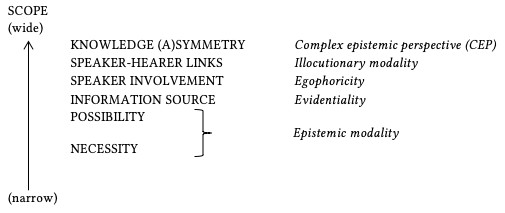
\includegraphics[width=\linewidth]{figures/grzech-2}
	\caption{Dimensions of the epistemic perspective domain (after \citealt[12]{Bergqvist2017})}\label{fig:kg2}
\end{figure}


As mentioned above, the notion of \emph{epistemic perspective} points to the fact that all the categories shown in Figure \ref{fig:kg2} are to some extent concerned with marking the different dimensions of epistemic access of the participants of discourse. From bottom to top, the different epistemic marking systems shown on the right-hand side are organised from the least to the most intersubjective. On the left-hand side, Figure \ref{fig:kg2} shows the different functional domains corresponding the epistemic marking systems shown on the right. The arrow corresponds to the levels of meaning, based on the assumptions that the categories at the bottom of the scale encode more propositional meaning, and hence have narrower scope, and the categories towards the top encode non-propositional meaning. The marking of complex epistemic perspective refers to the fully intersubjective systems, in the encoding of which the perspectives of both participants of the interaction are equally important. The composition of the domain presented in Figure \ref{fig:kg2} is based on a preliminary cross-linguistic survey, including the grammatical categories attested in a sample of languages which exhibit the exemplified epistemic marking systems (\citealt{Bergqvist2017}). 

The number of functional sub-domains – and corresponding grammaticalised marking systems – is bound to increase if other languages are taken into account. Examples of such systems could include the marking of engagement (cf. e.g. \citealt{Landaburu2007}), information status of discourse participants (cf. \citealt{SanRoque2008}), or the marking of epistemic primacy, discussed at length in this chapter. In Japanese, epistemic primacy is encoded by dedicated morphology, namely the marker \textit{yo} (\citealt{Hayano2011}). In the following sections, I show that epistemic primacy is also morphologically marked in Upper Napo Kichwa, where the distribution of epistemic authority between speaker and hearer is encoded by =\textit{mi} and =\textit{cha}. Therefore, at least for certain languages, including Upper Napo Kichwa, epistemic primacy should be considered one of the \emph{functional sub-domains} within the overarching domain of epistemic perspective. 


\subsubsection{Common Ground and focus}\label{s:kg1-3-4}

The remaining notions that need to be explained before I proceed to the analysis of the Upper Napo Kichwa enclitics =\textit{mi} and =\textit{cha} are Common Ground and focus, both pertinent to the study of information structure. I define them in turn below. The readers should keep in mind that the definitions provided here are not meant to tackle the conceptual complexity of the discussed notions in full detail. Rather, they are meant to provide basic definitions, so as to allow for a consistent, clear interpretation of the analysis presented in the following sections.

\textsc{Common ground} (henceforth CG) consists of information which is mutually known to be shared by the discourse participants (cf. e.g., \citealt{Stalnaker1974}; \citealt{Clark1996}). This information includes discourse referents interlocutors are familiar with, and ‘a set of propositions which the participants in the conversation mutually agree to treat as true for the purpose of the exchange’ (\citealt{Stalnaker1978}). CG constantly develops over the course of communication, and \cite{Krifka2007} points out that there are two aspects of CG relevant to communication: CG \textsc{content}, which includes all the truth-conditional information within the CG, and CG \textsc{management}, which indicates the way in which CG content should develop. Both CG content and CG management are shared between discourse participants. The aspects of information structure (henceforth IS) that have truth-conditional impact can be associated with CG content, and those relating to the pragmatic use of expressions – with CG management (\citealt[18]{Krifka2007}). Over the course of this chapter, I show that Upper Napo Kichwa discourse enclitics contribute to CG management, rather than to CG content.

As mentioned above, CG develops constantly in the process of communication. For this to occur, utterances need to contain not only information already known to both interlocutors, but also information known to the speaker, but new to the hearer, so that it can be added to CG in the process of communication. However, there are cognitive constraints on how much new information can be conveyed at a time. According to the \textsc{one new idea constraint} (\citealt{Chafe1987}; \citealt{Chafe1994}), for processing reasons, every clause in connected discourse can contain only one concept which falls under the scope of assertion: the focus of the clause. Clauses also contain presupposed content, and within it, expressions denoting referents the clause is about (cf. \citealt[127]{Lambrecht1994}). In IS terms, such a referent is the topic of the clause. Both topic and focus are relational notions. That is, no referent is inherently focal or topical. Rather, the topic or focus relation arises between discourse referents and propositions as a result of the speaker’s strategy of CG management. 


\section{Upper Napo Kichwa discourse enclitics: the paradigm}\label{s:kg2}

In this section I present the morphosyntactic paradigm of Upper Napo Kichwa discourse enclitics, of which both =mi and =cha form part. As mentioned in §‎\ref{s:kg1-2}, Upper Napo Kichwa is an exclusively suffixing language. Consequently, all the clitics found in the language are in fact enclitics. Moreover, all the enclitics attested in Upper Napo Kichwa are free, that is, they attach to hosts from any grammatical category, as long as their hosts function as phrasal heads.\footnote{In §\ref{s:kg1-2}, I mention that Upper Napo Kichwa has two main grammatical categories, nouns and verbs. Nonetheless, members of minor word classes, e.g., adverbs, can also function as phrasal heads/hosts for enclitics in Upper Napo Kichwa.}

The presence of free enclitics is attested in all described Quechuan varieties (cf. e.g., \citealt{Parker1969}; \citealt{Cole1982}; \citealt{Weber1986}; \citealt{Cusihuaman1976}), but most authors do not grant them a comprehensive description, focusing only on a few selected markers. In the Upper Napo Kichwa data collected to date, as many as fifteen free enclitics were attested (cf. \citealt[ch.3]{Grzech2016a}). Of those, nine were identified as \textsc{discourse (en)clitics}, that is, defined by \cite[37]{Spencer2012}) as clitics which express discourse functions, rather than inflectional categories. The occurrence of discourse enclitics is not conditioned by grammar, and hence no contexts were identified in which their occurrence would be required for the syntactic well-formedness of the clause. Rather, they are used to enhance discourse coherence by encoding “cues for interpretation, (…) emphasis, rhetorical effects, or the attitude of the speaker” (cf. \citealt[35]{Spencer2012}). Of the nine discourse enclitics in Upper Napo Kichwa, one, namely =\textit{ga}, seems to be associated with presupposed information (cf. \citealt[ch.4]{Grzech2016a}). The remaining eight markers – among them the two enclitics described in this chapter – associate with focal referents. These eight enclitics, along with their previous analyses, are listed in Table \ref{tab:kg1}. 

%TODO include references in table
\begin{table}[h]
\centering
\begin{tabularx}{\textwidth}{L{2cm}L{9cm}}
\hline
\textbf{=\textit{mi}}	
&	Validational (e.g., Cole 1982),	\\
			&	Direct evidential (Weber 1986; Floyd 1997; Faller 2002), 	\\
			&	Best possible ground marker (Faller 2002),	\\
			&	Focus marker (Muysken 1995; Cusihuamán 1976/2001; Sánchez 2010; 2015) 	\\
\hline
\textbf{=\textit{ma}}	
&	Emphatic equivalent of =\textit{mi} (Cole 1982)	\\
			&	Direct experience marker (Hintz \& Hintz 2014)	\\
			&	Marker of surprise (Faller 2002)	\\
			&	Impressive/emphatic marker (Cusihuamán 1976/2001)	\\
\hline
\textbf{=\textit{mari}}		&	Emphatic equivalent of =\textit{mi} (e.g., Cole 1982; Floyd 1997; Faller 2002)	\\
\hline
\textbf{=\textit{cha}}	&	Validational (Adelaar 1977; Cole 1982), 	\\
			&	Inferential/conjectural evidential (e.g., Weber 1986; Floyd 1997), 	\\
			&	Inferential/conjectural evidential and  epistemic modal (e.g., Faller 2002).	\\
\hline
	\textbf{=\textit{chari}}		&	Emphatic equivalent of =\textit{cha} (e.g., Faller 2002)	\\
\hline
	\textbf{=\textit{chu}}		&	Negation and polar question marker (e.g., Cole 1982; Weber 1989; Cusihuamán 1976/2001)	\\
\hline
	\textbf{=\textit{ta}}		&	Possible cognate of question marker -\textit{taq} (cf. Weber 1989).	\\
\hline
	\textbf{=\textit{tá}}		&	Not attested in other varieties / Verum focus marker	\\
\hline
\end{tabularx}
\caption{Focus-related discourse enclitics in Upper Napo Kichwa}\label{tab:kg1}
\end{table}


All of the enclitics listed in Table \ref{tab:kg1} occur on focal referents, and attach to their hosts word-finally, following all the inflectional morphology. However, apart from being associated with focus, they also play different roles in Upper Napo Kichwa discourse. For the sake of space, this chapter only concentrates on two of the markers listed above, =\textit{mi} and =\textit{cha}.

As mentioned above, all the Upper Napo Kichwa enclitics are syntactically non-obligatory, and the same applies to the two markers in question. In the parsed-and-glossed part of the Upper Napo Kichwa corpus, comprising 1537 turns, =\textit{mi} occurred in 5.9\% of the turns (n=96), and =\textit{cha} was even less frequent, occurring in 2.15\% of turns (n=33). This low frequency suggests that despite their association with focus, other discourse-related factors are decisive when it comes to the markers’ use in discourse. In the following sections, I explore these factors, including their epistemic primacy semantics and their role in CG management.  

\section{Quechuan evidential enclitics and the Upper Napo Kichwa “evidential” paradigm}\label{s:kg3}

As mentioned in the previous sections, in most other varieties of Quechua described to date, =\textit{mi} and =\textit{cha} are analysed as evidential markers encoding direct and conjectural/inferential evidence, respectively. In this section, I present the Quechuan evidential paradigm (\ref{s:kg3-1}‎) and present the analysis of =\textit{mi} and =\textit{cha} in other Quechuan varieties (\ref{s:kg3-2}), so as to contextualise the analysis of the Upper Napo Kichwa markers presented in §\ref{s:kg4}‎ and §‎\ref{s:kg5}. 

\subsection{The Quechuan evidential paradigm}\label{s:kg3-1}

Apart from the two markers described in this chapter, the evidential paradigm found in most Quechuan varieties also contains a third marker, encoding reportative evidence. This three-choice system is illustrated in (\ref{ex:kg1}) below with data from Cuzco Quechua, spoken in Peru (adapted from \citealt[122]{Faller2002}):

\begin{exe} 
\ex Cuzco Quechua\footnote{Language names are only included in examples from languages other than Upper Napo Kichwa.}\label{ex:kg1} 
\begin{xlist} 
	\ex Direct/Best possible ground\footnote{I explain the notion of ‘Best possible ground’ below.} =\textit{mi}\\
		\glll Parashanmi.\\
		para-sha-n=\textbf{mi} \\
		rain-\textsc{prog}-3=\textbf{\textsc{mi}} \\
		\trans ‘It is raining.’ [speaker sees that it’s raining]
	\ex Inferential/conjectural =\textit{chá}\\
		\glll Parashanchá.\\
		para-sha-n=\textbf{chá}.\\
		rain-\textsc{prog}-3=\textbf{\textsc{chá}}\\
		\trans ‘It is raining.’ [speaker conjectures that it’s raining]
	\ex Reportative =\textit{si}\\
		\glll Parashansi.\\
		para-sha-n=\textbf{si}.\\
		rain-\textsc{prog}-3=\textbf{\textsc{si}}\\
        \trans ‘It is raining.’ [speaker was told that it’s raining]	
\end{xlist}
\end{exe}

%TODO Hintz 2012a and 2012b > not same author!
The paradigm shown in (\ref{ex:kg1}) is attested in most described Quechuan languages. However, some varieties diverge from it, offering the speakers more choices. South Conchucos Quechua (QI) is reported to have five evidential markers (Daniel J. \citeyear{DanielHintz2012}; \citeyear{Hintz2014}). Six markers have been described for Sihuas Quechua (QI) (Dianne \citeyear{DianneHintz2012}; \citealt{Hintz2014}) and Huamalíes Quechua (\citealt{Howard2012}), both closely related to South Conchucos. In these varieties, the speaker’s choice of evidential is influenced not only by the type of evidence, but also by the distribution of knowledge between discourse participants.  All these systems have the direct, indirect and reportative markers. In addition, South Concuchos has markers asserting mutual knowledge and indicating shared conjecture (\citealt{Hintz2014}). Sihuas has a system of three contrastive pairs, indicating the distinctions between individual and mutual knowledge, individual and shared conjecture and individual knowledge from report vs generalised knowledge from report (\citealt{Hintz2014}). In Humalíes, the non-standard markers indicate speculation, affirmation of knowledge co-constructed by the speaker and the hearer, and negation of such knowledge\footnote{In \citeauthor{Howard2012}'s (\citeyear{Howard2012}) terms, co-constructed knowledge results from the exchange of information between the speaker and the addressee. This is different from \citeauthor{Hintz2014}'s (\citeyear{Hintz2014}) ‘shared knowledge’, understood as knowledge shared by participants, acquired either through a linguistic exchange, or through a shared non-linguistic experience. The latter understanding is more in line with widely accepted definitions of Common Ground.} (\citealt{Howard2012}). In the above systems, the markers do not correspond strictly to source of information – the use of \textsc{individual} vs \textsc{shared knowledge markers} is also influenced by the speaker’s opinion about whether she has epistemic authority over the information conveyed (\citealt[8]{Hintz2014}). Epistemic authority in particular is relevant to the description of the ‘evidential’ markers in Upper Napo Kichwa, as I show in §‎\ref{s:kg4}.

In the varieties discussed above, the evidential paradigm consists of three or more markers. However, in some varieties, including Imbabura Quechua (QII) (\citealt[164--165]{Cole1982}), spoken in the Ecuadorian Highlands\footnote{\cite[165]{Cole1982} observes that while the marker -\textit{shi} is attested in Imbabura, it seems to have undergone semantic shift from marking hearsay to marking speculation.}, and Upper Napo Kichwa, described here, reports are marked periphrastically by means of the verb \textit{ni}- (‘say’) rather than by the use of a dedicated marker. Interestingly, the reportative marker is attested in Pastaza Quichua (QII) (\citealt{Nuckolls1993}; \citealt{Nuckolls2012}), which is related to Upper Napo Kichwa more closely than the highland Imbabura variety.

In the Upper Napo Kichwa data, the reportative marker  seems to have been replaced by a periphrastic construction, whereby the verb of speech \textit{ni}- (‘say’) is used in all hearsay/reportative contexts as a marker of reported speech, and the speech complements are often marked by the enclitic =\textit{mi} (see examples (\ref{ex:kg5}) in §‎\ref{s:kg3-2} and (\ref{ex:kg22}) in §‎\ref{ex:kg6}). Given that the reportative enclitic is not attested in the Upper Napo Kichwa data, I limit the discussion here to the direct and conjectural/inferential markers.


\subsection{Analyses of =\textit{mi} and =\textit{cha} in other Quechuan varieties}\label{s:kg3-2}

The analyses of =\textit{mi} as a direct evidential in different dialects of Quechua point to the fact that it can mark propositions for which the origo has direct, sensory evidence. However, a broader definition of the marker’s semantics was proposed by \cite{Faller2002}, in order to reflect the fact that the direct/sensory access analysis cannot account for all uses of =\textit{mi} in Cuzco Quechua (QII). \cite{Faller2002} analysed =\textit{mi} as the marker of \textsc{best possible ground} (henceforth BPG). BPG corresponds to direct evidence if the information in question belongs to the speaker’s own life experience. However, in case of encyclopedic knowledge, which tends to be learnt from authority rather than through direct experience, the BPG can correspond to reportative evidence. Under \citeauthor{Faller2002}’s view, having the best possible source of information is a necessary, but not sufficient condition for making a =\textit{mi}-marked statement. In order to felicitously use =\textit{mi}, the speaker needs to have the BPG for making a statement. To have the BPG, apart from having the best possible source of information, the speaker also needs to have assimilated the proposition into his network of beliefs (\citealt[140--141]{Faller2002}).

As for =\textit{cha}, the marker has previously been analysed as a “conjectural” (\citealt{Weber1986}; \citealt{Faller2002}), “inferential” (\citealt{Floyd1997}) or “dubitative” (\citealt{Muysken1995}) marker in the different Quechuan varieties. Despite the different labels, in all the varieties for which it has been described, the marker is reported to cover indirect evidence based both on reasoning and conjecture. \cite[ch.5]{Floyd1997} analyses the meaning of the Wanka Quechua -\textit{chr(a)} as prototypically indicating that a given utterance is an inference. According to \citeauthor{Floyd1997}, the prototypical meaning of the marker is “attenuation in the domain of commitment”, which “equates non-incorporation into reality (…) and is encoded in terms of likelihood values” (\citealt[106]{Floyd1997}). He further claims that the non-prototypical uses of =\textit{chr(a)} have to do with attenuation in other domains, including e.g., the “psychological distance between the hearer and the proposition”.

Although \citeauthor{Floyd1997} does not explicitly refer to epistemic modality, the fact that he analyses the marker as encoding commitment to the likelihood of propositions amounts to an evidential/modal analysis, which is the one that \citeauthor{Faller2002} (\citeyear{Faller2002}; \citeyear{Faller2007}) proposes in her work on Cuzco Quechua (QII). According to Faller, the conjectural marker is the only CQ evidential that is both an evidential and an epistemic modal. The evidential meaning of =\textit{chá} is to indicate that the speaker “bases his or her statement on a mental process”, be it inference, conjecture, guesswork or any other process involving reasoning (\citealt[176]{Faller2002}). However, if  the speaker bases her statement on partial direct evidence, -\textit{chus hina} – a marker which occurs in complementary distribution with other evidential enclitics (\citealt{Faller2006}) – is preferred over -\textit{chá}. Consider the following example from Cuzco Quechua:


\begin{exe}
	\ex Cuzco Quechua\label{ex:kg2}
	\begin{xlist}
		\ex 
		\glll ?Unqusqachá kashanman.\\
		unqu-sqa-chá ka-sha-n-man\\
		sick-\textsc{prt}-\textsc{conj} be-\textsc{prog}-3-\textsc{cond}\\
		\trans ‘She may be sick.’ [Context: Marya looks very pale.]
		\ex 
		\glll Unqusqachus hina kashanman.\\
		unqu-sqa-chus hina ka-sha-n-man\\
        sick-\textsc{prt}-\textsc{res} {} be-\textsc{prog}-3-\textsc{cond}\\
        \trans ‘She appears to be sick.’ (Faller 2007: 4)
	\end{xlist}
\end{exe}

The marker -\textit{chus hina}/\textit{chu shina} means roughly ‘I guess’/‘I think’/‘apparently’ (\citealt[3]{Faller2006}). In Cuzco Quechua, -\textit{chá} cannot be used if the speaker is certain that the proposition is true or false, even if she arrived at that conclusion through reasoning (\citealt[5]{Faller2007}). This supports the epistemic modal analysis of -\textit{chá}. For a -\textit{chá}-marked proposition to be felicitous, the speaker needs to believe in the possibility that the proposition expressed is true, as well as having arrived at that belief by her own reasoning.

The analyses of =\textit{mi} and =\textit{cha} presented above cannot be applied to their Upper Napo Kichwa cognates. In the case of =\textit{mi}, neither the ‘direct evidential’ nor the BPG analysis account for all uses of the marker. The following examples show that the marker can be used in statements based on different evidence types, including direct/visual source of information, as in (\ref{ex:kg3}), inference or conjecture, as in (\ref{ex:kg4}) and (\ref{ex:kg5}), or reportative evidence, as in (\ref{ex:kg6}):

\begin{exe}
	\ex Direct/visual\label{ex:kg3}\\
	\glll Tamyawmi.\\
	tamya-w=\textbf{mi}\\
	rain-\textsc{prog}=\textbf{\textsc{mi}}\\
	\trans ‘It is raining’ [uttered while observing the rain]. [el\_21092014\_01 003]
\end{exe}

\begin{exe}
	\ex Inference/conjecture\label{ex:kg4}\\
	\glll [Cesar] mingamami rishka.\\
	[Cesar] minga-ma=\textbf{mi} ri-shka\\
	[Cesar] collective.work-\textsc{dat}=\textbf{\textsc{mi}} go-\textsc{ant}\\
	\trans ‘[Cesar] went to the minga’ [the speaker has just arrived at C’s home. C. is not there, it’s the day of the minga, and the speaker knows C. always participates in community events] [el\_21092014\_01 051]
\end{exe}

\begin{exe}
	\ex Inference/conjecture\label{ex:kg5}\\
	\glll Ñuka yaya shamuwmi yachin.\\
	ñuka yaya shamu-w=\textbf{mi} yachi-n \\
	1\textsc{sg} father come-\textsc{prog}=\textbf{\textsc{mi}} seem-3\\
	\trans ‘It seems my father is coming.’ [speaker hears footsteps outside, and was expecting his father to come] [el\_21092014\_01 035]
\end{exe}

\begin{exe}
	\ex Reportative evidence\label{ex:kg6}\\
	\glll Rimawanun Saida ungushkami sirik nisha.\\
	rima-wa-nun Saida ungu-shka=\textbf{mi} siri-k ni-sha\\
	say-1\textsc{obj}-3\textsc{pl} \textsc{name} fall.ill-\textsc{ant}=\textbf{\textsc{mi}} stay-\textsc{nmlz} say-\textsc{coref}\\
	\trans ‘They tell me Saida is ill.’ [el\_25092014\_01 113]
\end{exe}

Example ‎(\ref{ex:kg3}) can easily be reconciled with the both the direct evidential and the BPG analysis of =\textit{mi}. Example (\ref{ex:kg6}), where =\textit{mi} is used within a reportative construction, could indicate that in this case =\textit{mi} can be analysed as a marker of BPG, as the fact which the speaker reports is not accessible to him directly, and thus the best possible evidence is that of a verbal report. However, according to the analyses presented above, examples (\ref{ex:kg4}) and (\ref{ex:kg5}) could not be marked by =\textit{mi} in any of the varieties of Quechua discussed there. Rather, they would be marked by =\textit{cha}, as in both cases the speaker arrives at the proposition expressed by the utterance by reasoning. Moreover, as shown below, the Upper Napo Kichwa =\textit{mi} is also felicitously used when the speaker cannot be certain of having the BPG:

\begin{exe}
	\ex Guesswork / Inference based on partial evidence\label{ex:kg7}\\
	\glll Lluki puramami rin, llukipurama...\\
	lluki pura-ma=\textbf{mi} ri-n lluki-pura-ma\\
	left side-\textsc{dat}=\textbf{\textsc{mi}} go-3 left-side-\textsc{dat}\\
	\trans ‘[the seed] goes to the left, to the left’ [el\_03102014\_01   076]
\end{exe}

The utterance in (\ref{ex:kg7}) comes from an elicitation session during which two participants watched recordings of a magician preforming six games of a three-shell game. In case of each game, they first watched it without the final part in which the location of the seed was revealed, and were asked to guess where the seed was. After they took their guesses, the same game was re-played again, this time with the finale, so that the participants could confront their guesses with reality.\footnote{This elicitation session is accessible online in the ELAR Upper Napo Kichwa deposit, under the following link: \url{https://elar.soas.ac.uk/Record/MPI1034554}.}  The participant who uttered (\ref{ex:kg7}) was guessing the location of the seed. He had already made several attempts at guessing where the seeds were located, each of them failed. Thus, the use of =\textit{mi} in (\ref{ex:kg7}) cannot be explained by the speaker’s certainty of having the BPG for the proposition. 
In §\ref{s:kg4}, I demonstrate that conversely to the direct evidence/BPG analysis, the epistemic primacy analysis of =\textit{mi} can account for all the examples given above.

The Upper Napo Kichwa =cha also does not lend itself well to the analyses proposed for its cognates. If it was in fact a conjectural/inferential marker, we would expect to find it in examples such as (\ref{ex:kg4}) and (\ref{ex:kg5}) above, which are, however, marked by =\textit{mi}. Moreover, =\textit{cha}-marked statements, when presented without further context, are always interpreted as interrogative, rather than declarative utterances. Consider:

\begin{exe}
	\ex \label{ex:kg8}
	\begin{xlist}
		\ex \label{ex:kg8a}
		\glll \#Tamiashkacha.\\
		 tamia-shka=\textbf{cha}\\
		rain-\textsc{ant}=\textbf{\textsc{cha}}\\
		\trans Intended meaning: ‘It rained/It must have rained’ [speaker haven’t seen the rain, but 	sees the ground is wet] [elicited]
		\ex  \label{ex:kg8b}
		\glll Tamiashkacha?\\
		tamia-shka=\textbf{cha}\\
        rain-\textsc{ant}=\textbf{\textsc{cha}}\\
        \trans ‘Has it rained? / It has rained, hasn’t it?’ [elicited]
	\end{xlist}
\end{exe}


The example (\ref{ex:kg8a}) was presented to consultants in an elicitation context, but they rejected it, proposing (\ref{ex:kg8b}) instead. If =\textit{cha} was a conjectural evidential, its use in a declarative statements would not be problematic, as suggested by evidence from other varieties of Quechua. 

Although =\textit{cha}-marked declaratives are not attested in elicitation, they do occur in naturalistic discourse, in utterances which can be interpreted as rhetorical questions, as in (9), or dubitative statements, as in (10):

\begin{exe}
	\ex Rhetorical question\label{ex:kg9}\\
	\glll Chiraygucha kay islamaga allí…\\
	chi-raygu=\textbf{cha} kay isla-ma=ga alli\\
	\textsc{d}.\textsc{dem}-\textsc{causal}=\textbf{\textsc{cha}}	 \textsc{p}.\textsc{dem}	 shore-\textsc{dat}=\textsc{top} good\\
	\trans ‘That would be why [the soil] is good on this shore’ [in\_01082013\_02 094]
\end{exe}

\begin{exe}
	\ex Dubitative\label{ex:kg10}\\
	\glll Ima shutiracha, Shangricha nijkuna akay...\\
	ima shuti-ta=\textbf{cha} Shangri=cha ni-k-kuna a-ka=y\\
	what name-\textsc{acc}=\textbf{\textsc{cha}} \textsc{name}=\textsc{cha} say-\textsc{nmlz}-\textsc{pl} \textsc{aux}-\textsc{pst}=\textsc{emph}.\textsc{int}\\
	\trans ‘What was his name, I think they called him Shangri…’ [in\_26052013\_02 132]
\end{exe}

Example ‎(\ref{ex:kg9}) is an excerpt from a conversation between two farmers, each of whom owns a plot of land on the shore of the Napo river, in roughly the same area. Although the speaker has first-hand knowledge about the quality of the soil on the shore, he still chooses to use =\textit{cha}, possibly because the plot of land under discussion belongs to the other farmer. Example ‎(\ref{ex:kg10}) further shows that Upper Napo Kichwa =\textit{cha} does not lend itself to the analyses proposed for its cognates. In this case, the speaker is an elderly woman trying to remember the name of a shaman she used to know in her youth. Her interlocutor is a young interviewer, who could not have possibly known the shaman. Here, =\textit{cha} is used despite the fact that the speaker has direct, though partial evidence for the proposition, as she knew the shaman in person. Thus, as shown in example ‎(\ref{ex:kg2}) above, in Cuzco Quechua that same example would have been marked by -\textit{chus hina}, rather than =\textit{cha}. As in case of =\textit{mi}, the occurrences of =\textit{cha} in the examples cited in this section cannot be accounted for by the evidential analysis, but can be explained if the marker is analysed as related to epistemic primacy. I discuss this analysis in detail in the following section.

\section{Epistemic primacy in Upper Napo Kichwa discourse}\label{s:kg4}

In the previous section, I have shown why the evidential analysis does not apply to the Upper Napo Kichwa enclitics =\textit{mi} and =\textit{cha}. Here, I spell out their analysis as markers of epistemic primacy. Firstly, I discuss the semantic contribution the two markers make to the clause (‎\ref{s:kg4-1}). Secondly, I explain how their epistemic primacy semantics can be reconciled with their association with focus (\ref{s:kg4-2}).

\subsection{Epistemic primacy semantics of =\textit{mi} and =\textit{cha}}\label{s:kg4-1}

As mentioned in §‎\ref{s:kg1-3-2}, epistemic primacy can be defined as a “relative right to know or claim” (\citealt{Stivers2011}). As such, the notion operates on a different level of discourse than that of evidence. Evidence or access to information by default relates to the text-external world. The same does not hold for epistemic primacy, which is more social or interpersonal. Conviction of having superior knowledge, or right to claim something, can of course also be grounded in the discourse-external reality, but that need not always be the case. Claims to superior knowledge can arise on the basis of subjective mental processes unrelated to external discourse contexts. Consequently, the notion of epistemic primacy is also broader. All the instances of the speaker having direct, sensory access to events can be explained as cases of evoking both direct evidence and epistemic authority/primacy, which arises by virtue of direct access to an event. However, cases such as the =\textit{mi}-marked guess in example ‎(\ref{ex:kg7}) can be explained by the speaker invoking epistemic primacy, but not by the direct evidence\footnote{In this particular case, “guesswork” could be regarded as inference based on partial evidence, rather than no evidence at all – despite the earlier erroneous guesses, the speaker might be conviced that this time their observation of the seed’s location is correct (thank you to Kasper Boye for pointing this out). This does not invalidate the main point of the argument – tha previous analyses do not hold for Upper Napo Kichwa =\textit{mi}. As discussed earlier, the Cuzco Quechua =\textit{mi} cannot be used in case of only partial direct evidence, where -\textit{chus hina} is preferred.} or \textsc{best possible ground} analysis (see §\ref{s:kg1-3-2}). 

As mentioned in §\ref{s:kg1-3-2}, an important component of the epistemic primacy meaning is its relative nature; The “relative right to know or claim” certain pieces of information arises as an interpersonal aspect of the context of the speech situation. Let us imagine a situation in which I explain the meaning of the Upper Napo Kichwa word \textit{ayllu} (‘family’/‘relatives’) to a fellow linguist, who works on another language family. In this encounter, I could safely assume epistemic primacy, since I am more qualified to talk about Quechuan than my colleague. The knowledge about Quechuan languages falls within my \textsc{territory of information} (cf. \citealt{Kamio1997}). However, if I were discussing the meaning of the same lexeme with any native speaker of Upper Napo Kichwa, it would be them, not me, who would hold epistemic primacy, by virtue of their native knowledge of the Kichwa language and culture. It follows that to claim epistemic primacy we do not need to be extremely highly qualified, or even certain about the veracity of the proposition; we do need to assume however, that we are more qualified to voice an opinion than our interlocutor is. If we assume that the Upper Napo Kichwa =\textit{mi} encodes epistemic primacy, examples of its use in utterances ‎(\ref{ex:kg3}) to ‎(\ref{ex:kg7}) given in §‎\ref{s:kg1-3-2} can all be accounted for. 

Another aspect of the meaning of =\textit{mi} which was not mentioned so far is that it undergoes \textsc{origo shift}. That is, it is anchored to the speaker in declarative clauses, and to the hearer in interrogative clauses - hence the use of the term \emph{origo} rather than \emph{speaker} in reference to the source of epistemic authority indexed by =\textit{mi}.  Consider:

\begin{exe}
	\ex \label{ex:kg11}
	\glll Ñuka shuti anmi Karolina.\\
	ñuka shuti an=\textbf{mi} Karolina\\
	1\textsc{sg}	 name be=\textbf{\textsc{mi}} \textsc{name}\\
	\trans ‘My name is Karolina.’ [elicited]
\end{exe}

\begin{exe}
	\ex \label{ex:kg12}
	\glll Ima shutimi?\\
	ima	shuti=\textbf{mi}\\
	what	 name=\textbf{\textsc{mi}}\\
	\trans ‘What’s her name?’ [asking about the name of a third person.] [in\_20092013\_03   216] %TODO hyphenation problem!
\end{exe}

In (\ref{ex:kg11}), the speaker introduces herself, and it is clear that the epistemic authority to give this type of information lies exclusively with her. In case of (\ref{ex:kg12}), however, it is not the speaker but the hearer who is the source of epistemic authority. Origo shift is not a singular feature of the Upper Napo Kichwa epistemic marking - it occurs in a great many evidential/epistemic marking systems described to date (cf. e.g., \citealt{Hargreaves2005}).

I turn now to the semantics of the Upper Napo Kichwa =\textit{cha}. In the previous section, I have shown that it is not satisfactorily analysed as a conjectural/inferential evidential. Instead, I propose to analyse the marker as indicating the speaker’s lack of epistemic primacy. This means that by using =cha the speaker indicates not having the “relative right to know or claim”. This analysis is compatible with the examples ‎(\ref{ex:kg9}) and (\ref{ex:kg10}) above, since having no epistemic primacy is compatible with doubt. However, the use of the marker in example ‎(\ref{ex:kg8}), which demonstrates that in the absence of context, =\textit{cha}-marked utterances are interpreted as interrogatives, requires additional explanation, which I provide in §‎\ref{s:kg5}.

The examples of =\textit{cha} given so far do not provide sufficient evidence for claiming that the marker indicates lack of epistemic primacy, as they would also be permissible if the marker simply had a dubitative meaning. What differentiates the dubitative from the “lack of epistemic primacy” expression is that, by using the first, the speaker indicates that he considers the proposition in question as a possibility. In the latter case, the speaker indicates that he is not in position to evaluate the probability of the proposition. The Upper Napo Kichwa data suggest that this in fact the case. In §\ref{s:kg3-2}  I have shown that Upper Napo Kichwa dubitative statements are marked with the epistemic modal \textit{yachin} (seem-3), potentially accompanied with =\textit{mi}, rather than with =\textit{cha} (see example ‎(\ref{ex:kg5})). Consider:

\begin{exe}
	\ex \label{ex:kg13}
	\begin{xlist}
		\ex \label{ex:kg13a}
		\glll Yaya yachin, paywa yaya…\\
		 yaya yachi-n, pay-pa yaya\\
		father-3 seem-3 3\textsc{sg}-\textsc{gen} father\\
		\trans ‘It seems [he is the] father, his father…’ [el\_18092014\_02 028]
		\ex  \label{ex:kg13b}
		\glll Yaya yachin, paywa yayacha…[?]\\
		yaya yachi-n, pay-pa yaya=\textbf{cha}\\
        father seem-3 3\textsc{sg}-\textsc{gen} father=\textbf{\textsc{cha}}\\
        \trans ‘It seems [he is the] father, isn’t he his father?/is he his father?’ [elicited]
	\end{xlist}
\end{exe}

The difference between (\ref{ex:kg13a}) and (\ref{ex:kg13b}) lies in the fact that in example (‎\ref{ex:kg13a}) speaker presents his own point of view, supposing that the farmer from the “Pear story” video (\citealt{Chafe1980}) is the father of the boy who comes over to steal the fruit. In (\ref{ex:kg13b}), the point of the utterance is different - the speaker first expresses a supposition that the man in the film is the boy’s father using the epistemic modal, and then acknowledges the lack of “right to claim”, turning to the addressee for the evaluation of the proposition. Examples (\ref{ex:kg14}) and (\ref{ex:kg15}) further support the claim that =\textit{cha} encodes lack of epistemic authority, rather than doubt:

\begin{exe}
	\ex \label{ex:kg14}
	\glll Mana yachani, imara\textbf{cha} ranga rawn…\\
	mana yacha-ni ima=ta=\textbf{cha} ra-nga ra-w-n\\
	\textsc{neg}   know-1  what=\textsc{int}=\textbf{\textsc{cha}} do-\textsc{fut} \textsc{aux}-\textsc{prog}-3\\
	\trans ‘I don’t know, what will he do…’ [about the boy in the “Pear story”] [in\_24092014\_01 026]
\end{exe}

\begin{exe}
	\ex \label{ex:kg15}
	\glll Mayma\textbf{cha} rinun, payna....Payna wasima rinawn yachin.\\
	may-ma=\textbf{cha} ri-nun payguna  payguna wasi-ma ri-nun yachi-n\\
	where-\textsc{dat}=\textbf{\textsc{cha}}  go-3\textsc{pl} 3\textsc{pl} 3\textsc{pl} house-\textsc{dat}  go-3\textsc{pl}  seem-3\\
	\trans ‘Where are they going. It seems they are going home…’ [el\_24092014\_02 028]
\end{exe}

In (\ref{ex:kg14}) and (\ref{ex:kg15}) =\textit{cha} occurs on interrogative pronouns in rhetorical content question, rather than marking propositions the veracity of which is not evident to the speaker, as a dubitative marker would. This is clear in (\ref{ex:kg15}), where the first clause of the utterance is marked with =\textit{cha} to show the lack of epistemic authority, and it is only in the second clause that the speaker makes a supposition, marking it with \textit{yachin} (seem-3). The above examples support the analysis of the marker as indicating that by using it the speaker assumes the position of lacking the knowledge necessary to evaluate its veracity.

There are two other important aspects of the meaning of =\textit{cha} which should be mentioned here. Firstly, unlike =\textit{mi}, the Upper Napo Kichwa =\textit{cha} does not undergo origo shift; the “lack of epistemic primacy” is always anchored to the speaker, irrespective of whether the utterance is interrogative or declarative. The research to date does not suffice to explain why this is the case.\footnote{The currently available data suggest that unlike =\textit{mi}, the meaning of is not =\textit{cha} not assign epistemic primacy to a particular participant of the interaction. Rather, it serves to indicate that the speaker does not hold it. This aspect of analysis needs to be developed in more detail, but it would explain why =\textit{cha} does not partake in origo shift (thank you to Henrik Bergqvist for this observation).} Further research is also needed to clarify the motivations speakers when they choose to use =\textit{mi} and =\textit{cha} in questions. It also remains to be established whether such choices are motivated by the content of the utterance, the epistemic context of discourse, or considerations related to politeness. Initial observations indicate that speakers resist using =\textit{mi} when asking questions concerning the addressee. In second person interrogatives =\textit{cha} or the negative/interrogative marker =\textit{chu} are strongly preferred; When I tried uttering declarative clauses with second person subject, my interlocutors corrected me, suggesting that what I wanted to say was actually a =\textit{chu} or =\textit{cha}-marked question. As shown in (\ref{ex:kg12}) above, the use of =\textit{mi} is not an issue in third person questions.

Lastly, it is important to note that the “lack of epistemic primacy” meaning does not always entail that the speaker’s epistemic access is inferior to that of the interlocutor. The examples (\ref{ex:kg13}) through (\ref{ex:kg15}) above suggest that =\textit{cha} is used in discourse in such contexts, and this is most often the case. However, this is not the case in (\ref{ex:kg10}), repeated below for the sake of clarity:

\begin{exe}
	\exr{ex:kg10} Dubitative\\
	\glll Ima shutiracha, Shangricha nijkuna akay...\\
	ima shuti-\textbf{ta}=\textbf{cha} Shangri=\textbf{cha} ni-k-kuna a-ka=y\\
	what name-\textsc{acc}=\textbf{\textsc{cha}} \textsc{name}=\textbf{\textsc{cha}} say-\textsc{nmlz}-\textsc{pl} \textsc{aux}-\textsc{pst}=\textsc{emph}.\textsc{int}\\
	\trans ‘What was his name, I think they called him Shangri…’ [in\_26052013\_02 132]
\end{exe}

As mentioned above, in this case the speaker is trying to remember an event from her youth, and marks the propositions she is not sure about with =\textit{cha}. However, her interlocutor is a young person who could not have known the shaman whose name the speaker is trying to remember. Therefore, a more plausible analysis is that the speaker uses =\textit{cha} to indicate that she does not have epistemic primacy in this case, although as the narrator and witness of the events she is recounting, she could be expected by the interlocutors to have it. Although examples like this one need further analysis, they are still in line with the main point presented here – that the Upper Napo Kichwa =\textit{cha} can be analysed as a marker of “lack of epistemic primacy” on the part of the speaker.

In this section, I have shown that the two Upper Napo Kichwa markers described in this chapter, namely =\textit{mi} and =\textit{cha}, can be analysed as encoding “epistemic primacy of the origo” and “lack of epistemic primacy of the speaker”, respectively. In the following section, I discuss the relationship between the markers’ semantics and their association with focus. 


\subsection{Epistemic primacy and focus}\label{s:kg4-2}

In Table \ref{fig:kg1} (§\ref{s:kg2}), I show that the cognates of the markers =\textit{mi} and =\textit{cha} in other Quechuan  varieties were often analysed as focus marker (cf. e.g., \citealt{Muysken1995}; \citealt{Sanchez2010}; \citeyear{Sanchez2015}). In the same section, I mention that in Upper Napo Kichwa, =\textit{mi} and =\textit{cha} seem to be associated with focus, but are too infrequent to be plausibly analysed as focus markers. I have discussed the interaction of focus with =\textit{mi} and =\textit{cha} in detail elsewhere (\citealt[ch.4]{Grzech2016a}). Here, for the sake of space, I limit the discussion to those aspects of the markers’ association with focus that are relevant to describing the interdependence between their focus-related function and their epistemic primacy-related semantics.
 
The marker =\textit{mi} can occur in different types of focus structures, but it seems to only be obligatory for the felicity of utterances which contain contrastive focus. Consider:  

\begin{exe}
	\ex \label{ex:kg17}
	\glll Mana ñuka ushichu, ñuka warmimi / \#warmi\\
	mana ñuka ushi=chu, ñuka warmi=\textbf{mi} / \#warmi\\
	\textsc{neg}	 1\textsc{sg} daughter=\textsc{q}/\textsc{neg} 1\textsc{sg} woman=\textbf{\textsc{mi}} / \#woman\\
	\trans ‘[She is] not my daughter, [she is] my wife.’ [elicited]
\end{exe}

Contrastive focus, as understood here, exhibits two main properties: (1) having a set of identifiable alternatives (cf. \citealt{Kiss1998}; \citealt{Repp2010}) and (2) implying the rejection of those alternatives (\citealt[1336]{Repp2010}). Both apply to (\ref{ex:kg17}) above and (\ref{ex:kg18}) below, which the speakers also resisted accepting without =\textit{mi}:

 
\begin{exe}
	\ex \label{ex:kg18}
	\glll Mana atarikanichu, tianukallami.\\
	mana atari-ka=chu tia-nuka=lla=\textbf{mi}\\
	\textsc{neg} get.up-\textsc{pst}=\textsc{q}/\textsc{neg}  be-3\textsc{pl}.\textsc{pst}=\textsc{lim}=\textbf{\textsc{mi}}\\
	\trans ‘[(S)he] didn't stand up, they just sat [there]’ [el\_24112014\_01   041]
\end{exe}

The contrastive constructions exemplified in (\ref{ex:kg17}) and (\ref{ex:kg18}) are also corrective, that is, the alternatives to the focused constituent are not only identifiable, but also overt (cf. \citealt{Repp2010}).  Correction involves rejection of an alternative proposition that is currently under discussion, or which the hearer assumes to form part of CG. The =\textit{mi}-marked constituents are introduced to the CG in the aftermath of the rejection of the =\textit{chu}-marked alternatives. Consequently, in both cases, propositions which one of the speakers considered true before the exchange are rejected, and replaced with the new, =\textit{mi}-marked content. The fact that =\textit{mi} is required for the felicity of such constructions is fully compatible with the marker’s ‘epistemic primacy’ semantics. By uttering (\ref{ex:kg17}) and (\ref{ex:kg18}), the speaker contradicts a proposition the hearer held as true, and introduces a new one, the factuality of which was outside the interlocutor’s awareness. Hence, in both cases, it is the speaker who holds the epistemic primacy. This would explain the fact that =\textit{mi} is required for the felicity of this type of utterances. The marker can also occur in information focus structures, but consultants deem those equally permissible with and without =\textit{mi}. The non-obligatoriness of the marker in such contexts plausibly stems from the fact that in the case of information focus it is not always clear - as it is in cases of corrective, contrastive foci - that the interlocutor was neither aware of, nor expecting\footnote{Expectation is another factor which seems to be relevant to the occurrence of =\textit{mi} in Upper Napo Kichwa. For reasons of space, I do not discuss is in detail here, but a discussion of its role in the distribution of =\textit{mi} is provided elsewhere (cf. \citealt[ch.6]{Grzech2016a}).}, the focal content of the utterance.

Let us compare the above to the correlation of focus with =\textit{cha}, which occurs only in information focus contexts. Consider the following exchanges: 


\begin{exe}
	\ex \label{ex:kg19}
	\begin{xlist}
		\ex \label{ex:kg19a}
		\glll Ayajcha panga?\\
		ayaj=\textbf{cha} panga\\
		bitter=\textbf{\textsc{cha}}   leaf\\
		\trans ‘[is it a] bitter leaf?’
		\ex  \label{ex:kg19b}
		\glll Ayajtá\\
		ayaj=\textbf{tá}\\
        bitter=\textbf{\textsc{tá}}\\
        \trans ‘[it IS]  bitter’ [in\_05092014\_01   033-34]
	\end{xlist}
\end{exe}

\begin{exe}
	\ex \label{ex:kg20}
	\begin{xlist}
		\ex \label{ex:kg20a}
		\glll Shindzi waskachá?\\
		shindzi waska=\textbf{cha}\\
		strong	string=\textbf{\textsc{cha}}\\
		\trans ‘[Is] the string strong?’
		
		\ex  \label{ex:kg20b}
		\glll Shindzimi\\
		shindzi=\textbf{mi}\\
        strong=\textbf{\textsc{mi}}\\
        \trans ‘[It is] strong’ [in\_20092013\_01    186-87]
	\end{xlist}
\end{exe}

In the question-answer pairs in (\ref{ex:kg19}) and (\ref{ex:kg20}), =\textit{cha} is used to indicate the focus of the interrogative clauses. In the corresponding answers, the focus is marked with the verum focus marker =\textit{tá} and with =\textit{mi}, respectively. The enclitic =\textit{cha} is not syntactically obligatory in the contexts shown above, but (quasi-)interrogatives are the most frequent context of its use. The fact that it tends to indicate information focus in rhetorical and confirmation questions is compatible with its “lack of epistemic primacy” semantics; marking the focus of interrogative utterances is tantamount to highlighting the portion of the utterance about which the speaker does not have sufficient knowledge. Hence, he is requesting more information from the addressee. Therefore, highlighting focus in dubitative/interrogative contexts and marking the speaker’s “lack of epistemic primacy” can be regarded as complementary aspects of the discourse function of =\textit{cha}.

\section{Epistemic primacy and Common Ground management}\label{s:kg5}

The discussion so far suggests that both =\textit{mi} and =\textit{cha} are polyfunctional markers, encoding meanings related epistemic primacy and associated with the IS category of focus. Consequently, a question that emerges is whether these two aspects of meaning could be considered jointly, so as to arrive at a unified analysis of their function in discourse. In the paragraphs that follow, I propose that such an analysis is possible if we take the notion of Common Ground into account.

In §‎\ref{s:kg1-3-4}, I defined the notions of \textsc{common ground} (CG) and CG \textsc{management}. I mentioned that CG develops constantly over the course of communication. Its content expands as the interlocutors put forward new propositions, which they mutually agree to treat as true for the purpose of the exchange (cf. e.g., \citealt{Stalnaker1974}). However, CG consists not only of its truth-conditional content, but also of CG management, that is, linguistic devices indicating how CG should develop – what propositions should be added to it, and at which point in the conversation. The discussion in the following paragraphs is underpinned by another important assumption: that any update in the CG results from solving a \textsc{question under discussion} (henceforth QUD) (cf. \citealt{Asher1993}; \citealt{Matic2015}). QUDs are introduced into discourse to advance communication, often by means of interrogative clauses which require an answer. QUDs influence the development of the CG content by directing the communicative exchange towards saturating certain propositions, so that they can then be added to CG.

As mentioned above, the development of CG is also informed by expressions which contribute to CG management, rather than content. These type of expressions are typically non-truth conditional; they do not add to the proposition expressed, but rather constitute processing clues for the interlocutors, indicating whether and how certain propositions could be integrated into the CG content. I propose that the Upper Napo Kichwa enclitics discussed in this chapter belong to this class of expressions, with the epistemic primacy and information-structural aspects of their meaning contributing to their overarching function of CG management.

Although Quechuan epistemic/evidential markers have not been analysed in this way before, the idea that epistemic meanings and IS meanings are related to each other is not a new one. \cite[3]{Kamio1997} pointed out a conceptual relation between the \textsc{territories of information} and IS, as both relate to “the character of information expressed in natural language”. In Quechuan literature, these relations also have not gone without notice. \cite{Hintz2017} observe that “the inter-subjective nature of certain evidential systems” invites discussion of how evidentiality relates to CG. In her analysis of Cuzco Quechua evidentials, \cite{Faller2002} also mentions in passing that evidential marking is related to IS. In some previous studies (e.g., \citealt{Muysken1995}), the focus-related and evidential functions of the enclitics were acknowledged, although the relation between the two was not explained.

Upper Napo Kichwa =\textit{mi} and =\textit{cha} can be analysed as markers of CG management not only because of their meaning, but also because of the type of contribution they make to the proposition expressed. Both markers are non-truth conditional, which is confirmed by the fact that their contribution to the propositions expressed by the utterances in which they occur cannot be negated (for discussion, see \citealt[ch.5]{Grzech2016a}; \citeyear{Grzech2016b}). It follows that they cannot contribute to the CG content, which is truth-conditional by definition.

Let us discuss the CG management function of =\textit{mi} on the basis of is occurrence in declarative clauses, where the origo is tantamount to the speaker. As mentioned previously, the speakers use =\textit{mi} not only to indicate focus, but also to assert their epistemic primacy. In doing so, they highlight information as congruent with their own world knowledge, but not necessarily with that of the hearer. Consequently, the use of =\textit{mi} indicates that the speaker has information that is sufficient to resolve a certain QUD, and that this information is not shared with the interlocutor. The association of =\textit{mi} with contrastive focus is congruent with this analysis; In examples (\ref{ex:kg17}) and (\ref{ex:kg18}), the contrastive focus associated with =\textit{mi} was also corrective. A correction implies that the speaker assumes being the only participant of discourse who knows how to answer the current QUD. Consequently, the procedural meaning of =\textit{mi}, integrating both epistemic primacy and focus association, is to encourage the hearer to accept the =\textit{mi}-marked information as part of CG, despite the misgivings they might have about it. Consequently, the marker is a CG-management device, the function of which is to accelerate the integration of a certain proposition into CG. This is illustrated in (\ref{ex:kg21}) with an exchange that took place between myself (A) and a good friend of mine (B), when we talked about whether I would be able to prefer \textit{chicha}, a traditional drink made from manioc:

\begin{exe}
	\ex \label{ex:kg21}
	\begin{xlist}
		\ex \label{ex:kg21a}
		\glll Mana  ushani!\\
		mana   usha-ni\\
		\textsc{neg} can-1\\
		\trans ‘I cannot [make chicha]!’
		
		\ex  \label{ex:kg21b}
		\glll Ushanguimi!\\
		usha-ngui=\textbf{mi}\\
        can-2=\textbf{\textsc{mi}}\\
        \trans ‘Yes you can’ [attested]
	\end{xlist}
\end{exe}

In the example above, my friend corrected me, using a =\textit{mi}-marked utterance to dispel my doubts about my capability of preparing the drink. In this specific context, the use of =\textit{mi} with second person subject is not aimed to undermine my authority over my own actions or skills – rather, my friend wanted to emphasise the fact that she knows I am skilled, and she also knows how to make \textit{chicha}. She used the =\textit{mi}-marked assertion as form of encouragement, urging me to re-assess my skills.

The function of =\textit{cha} as a CG management device is a mirror-image of the function of =\textit{mi}. As discussed above, the Upper Napo Kichwa =\textit{cha} is associated with information focus and indicates that the speaker renounces epistemic primacy. Consequently, in terms of CG development, the use of =\textit{cha} indicates that the speaker does not have the information sufficient to answer the current QUD, and that input is needed from the hearer to integrate the =\textit{cha}-marked proposition into CG. This explains why, as shown in example (\ref{ex:kg8}), =\textit{cha}-marked propositions tend to be interpreted as interrogatives in the absence of further context. It is also congruent with the association of =\textit{cha} with information focus, as the enclitic attaches to that portion of the utterance that requires saturation in subsequent discourse. Consequently, the procedural meaning of =\textit{cha} in terms of CG management is to indicate that the current QUD is not yet solved, preventing the hearer from accepting the proposition as part of CG without further elaboration. This was shown in examples (\ref{ex:kg19}) and (\ref{ex:kg20}) above. 

In this section, I have shown that the two aspects of the semantics of =\textit{mi} and =\textit{cha} discussed in the previous parts of this chapter can be considered jointly, if we analyse the enclitics as markers of CG management. This suggests that rather than referring to them as markers of epistemic primacy associated with focus, they can be analysed as (part of) a morphosyntactic paradigm the main function of which is to manage the CG. In the following section, I show how this proposal can be integrated into a broader, cross-linguistic functional domain of \textsc{epistemic perspective}. 


\section{Common Ground management and the epistemic perspective domain}\label{s:kg6}

In §\ref{s:kg1-3-3}, I introduced the notion of the domain of \textsc{epistemic perspective} (\citealt{Bergqvist2017}), which brings together epistemic marking systems attested in various languages, proposing that they share a “functional space” in the grammar. The structure of the domain as proposed by Bergqvist was shown in Figure \ref{fig:kg2} in §\ref{s:kg1-3-3}‎, and is repeated below with minor modifications, incorporating the sub-domain of CG management:

%TODO Figure 4
\begin{figure}
abc
\todo[inline]{missing figure}
\caption{Dimensions of the epistemic perspective domain (based on \citealt[12]{Bergqvist2017})}
\label{fig:kg4}
\end{figure}

The placement of CG management shown in Figure \ref{fig:kg4} is based on the semantics of the Upper Napo Kichwa CG management markers; As shown in §‎\ref{s:kg4}, the Upper Napo Kichwa CG-managing enclitics indicate knowledge (a)symmetry between discourse participants, and hence are related to the category of \textsc{knowledge asymmetry}.

\cite{Bergqvist2017} based the bottom-to-top ordering of the different sub-domains of epistemic perspective on the assumption that the more intersubjective meanings correspond to a wider scope of linguistic expressions. This has been confirmed in the literature on grammaticalisation (\citealt{Traugott1995}; \citeyear{Traugott2003}; \citeyear{Traugott2010}; \citeyear{Traugott2012}; \citealt{Traugott2002}), including grammaticalisation of discourse markers (\citealt{Traugott1995}) and deictic elements, such as demonstratives (e.g., \citealt{Kratochvil2011}). \citeauthor{Traugott2010} (e.g., \citeyear{Traugott2010}) observes that subjectified elements tend to appear at the periphery of the constituent or clause. This observation applies both to Upper Napo Kichwa CG management markers, and to evidentials in other Quechuan varieties (e.g., \citealt{Muysken1995}; \citealt{Sanchez2015}).

Although I grouped the markers of CG management together with the marking of \textsc{complex epistemic perspective} (CEP) on the basis of both sub-domains relating to knowledge (a)symmetries, it remains unclear how CG management markers relate to CEP. Bergqvist characterises CEP as a subtype of multiple perspective (cf. \citealt{Evans2005}), in which “one perspective [is] embedded in another” (\citealt[6]{Bergqvist2017}). In Upper Napo Kichwa, =\textit{mi} – but not =\textit{cha} – can be embedded under verbs of speech and thinking, and thus participate in constructions which could be define as encoding multiple perspective. Such constructions are used to convey reports of other speakers’ utterances, as well as in in self-corrections. Consider:

\begin{exe}
	\ex \label{ex:kg22}
	\glll Muyura pitiwn…ima… Coco… Mana, cocomi [an] nini, cocochá…\\
	muyu-ta 	piti-w-n… ima… coco... mana coco=\textbf{mi} [a-n] ni-ni...   coco=\textbf{cha}...\\
	fruit-\textsc{acc} 	cut-\textsc{prog}-3 what coconut \textsc{neg} coconut=\textbf{\textsc{mi}} [cop-3] say-1 coconut=\textbf{\textsc{cha}}\\
	\trans ‘He is cutting [harvesting] fruit….what…[It’s a] coconut…No, I said “coconut”… [but is it a] coconut?’ [el\_24092014\_03   003-5]
\end{exe}

In (\ref{ex:kg22}), the speaker’s previous opinion about the type of fruit harvested in the “Pear story” video is embedded in the utterance conveying her current opinion. As such, the example could be analysed as an instance of CEP. Note that =\textit{cha} is also used in (\ref{ex:kg22}), but not within the complex perspective construction - the speaker marks her new opinion with that enclitic, having realised she is not able to name the fruit she is seeing.

In the light of the above discussion, the tentative positioning of the category of ‘CG management’ in the vicinity of CEP seems to be accurate. However, it requires further research into the scope of the Upper Napo Kichwa CG management markers. As mentioned above, the bottom-to-top ordering of the different sub-domains in Figure \ref{fig:kg4} is based on the assumption that the scope of the linguistic expression of these domains is narrow at the bottom and gets wider towards the top. Consequently, the expressions of CEP are supposed to scope over all the other types of markers. The scope properties of =\textit{mi} and =\textit{cha} need to be thoroughly investigated before a definite decision on the placement of the sub-domain of CG management can be made.\footnote{The scope of the markers is not discussed in this chapter, but I do tackle it to some extent in my previous work (\citealt[ch.5]{Grzech2016a}). Preliminary investigation shows that =\textit{mi} can be embedded under verbs of speech and thinking, and under certain modals, but not under negation. The marker =\textit{cha}, on the other hand, was not attested in embedding contexts. Both markers are ungrammatical with grammatically marked imperatives.}

Consequently, the discourse-semantic considerations presented above need to be investigated in more detail before definite conclusions can be reached about where CG management fits into the epistemic perspective domain. The relationships between the different sub-domains of epistemic perspective are also likely to be revised in the light of ongoing documentation of the world’s languages.

In sum, the Upper Napo Kichwa markers of CG management functionally and semantically fit within the functional domain of epistemic perspective postulated by \cite{Bergqvist2017}. The data from Upper Napo Kichwa also show that the domain is not complete in the shape in which it was proposed originally.\footnote{In the time between when this paper was first written and its going into print, a category of ‘engagement’ was put forward, which encompasses CEP and a broader range of phenomena related to epistemicity (\citealt{Evansetal2018}). While the analysis presented here does not take that development into account, it will have to be addressed in future studies of Upper Napo Kichwa epistemic marking.} 
Determining the place of the sub-domain of CG management within the general domain of epistemic perspective, as well as its relationship with other sub-domains, requires further, cross-linguistic research. In this context, the study of the Upper Napo Kichwa CG management enclitics brings us one step closer to describing and analysing the cross-linguistically valid functions and properties of epistemic marking systems across languages. 


\section{Summary and conclusions}\label{s:kg7}

Over the course of this chapter, the reader has become acquainted with the system of marking epistemic primacy in Upper Napo Kichwa, focusing on the enclitics =\textit{mi} and =\textit{cha}. I have shown that the two Upper Napo Kichwa enclitics belong to a larger paradigm, and that they can be analysed as marking epistemic primacy, and lack thereof, respectively. I have also shown that although the enclitics are associated with focus, they cannot be considered as focus markers. Consequently, I have demonstrated that the epistemic primacy semantics of the markers and their relation to focus can be brought together under one overarching function: CG management. Finally, I have discussed the place of CG management within the cross-linguistically valid epistemic perspective domain.

Numerous aspects of the Upper Napo Kichwa CG management markers remain to be investigated. First and foremost, although the considerations presented in this chapter help account for the occurrence of both enclitics in discourse, they are not sufficient to account for their non-occurrence. More factors, including (counter)expectation (cf. \citealt{Matic2015}), need to be taken into account in the future research into determining why the Upper Napo Kichwa enclitics are only attested in a very small percentage of the utterances in which they could grammatically occur. As for =\textit{cha}, it is still unclear what role politeness plays in motivating its occurrence in discourse. Furthermore, it remains to be explored how the analyses of epistemic marking systems in lesser-spoken languages such as Upper Napo Kichwa behave in discourse, and how their study can be integrated into the current of discourse analysis concerned with how epistemic meaning is expressed through discourse strategies and discourse structure, which has been on the rise since the publication of the seminal paper of \cite{Heritage2005}.

Nonetheless, the analysis of =\textit{mi} and =\textit{cha} presented here contributes to our current knowledge of epistemic marking systems in a variety of ways. The chapter adds our current knowledge of systems encoding epistemic meanings in Quechuan languages. As mentioned above, in most described Quechuan varieties, the cognates of the enclitics described in this chapter are analysed as evidential markers. Consequently, the analysis provided here adds to our cross-linguistic knowledge of evidential and related systems. The chapter also contributes to the description of epistemic primacy as a semantic category. Relatively little work has been done cross-linguistically on morphosyntactic systems encoding epistemic primacy (cf. e.g., \citealt{Stivers2011}; \citealt{Hayano2011}). As a result, the description of the Upper Napo Kichwa system contributes to what we know about the category’s cross-linguistic properties. The preliminary analysis of the relation of the Upper Napo Kichwa epistemic primacy markers to CG management in discourse, and to the epistemic perspective domain (\citealt{Bergqvist2017}) make the analysis presented here relevant to the study of linguistic devices encoding epistemic meaning in the cross-linguistic perspective.

\section*{Acknowledgments}

I would like to acknowledge the generous support granted to this research by ELDP (Endangered Languages Documentation Programme, grant number IGS0166). The data resulted from the ELDP-financed documentation project were deposited in the ELAR archive and can be accessed here: \url{https://elar.soas.ac.uk/Collection/MPI849403}. 

I would like to thank Lydia Chimbo and her family for giving me a home away from home in Ecuador, and all the inhabitants of Nuevo Paraíso for supporting the documentation project. In particular, I would like to acknowledge the work and support of Nilo Andy, Jacobo Chimbo and Wilma Aguinda. Lastly, thank you to two anonymous reviewers and to the editors of this volume for their comments and suggestions. All shortcomings of this work remain my own. 
 
 
\section*{Abbreviations}
\begin{tabularx}{.45\textwidth}{lL{4cm}}
\textsc{1} & first person\\ 
\textsc{3} & third person\\ 
\textsc{1obj} & 1st person singular object\\
\textsc{acc} & accusative\\ 
\textsc{ant} &anterior\\  
\textsc{aux} & auxiliary\\  
\textsc{causal} & causalis\\ 
\textsc{cond} & conditional\\  
\textsc{conj} & conjectural\\ 
\textsc{cop} & copula\\ 
\textsc{coref} & coreference\\ 
\textsc{d} & distal\\ 
\textsc{dat} & dative\\ 
\textsc{dem} & demonstrative\\  
\textsc{emph} & emphatic\\ 
\textsc{fut} & future\\ 
\textsc{gen} & genitive\\  
\textsc{lim} & limitative\\ 
\textsc{int} & interrogative\\ 
\textsc{name} & proper name\\ 
\textsc{neg} & negative\\ 
\textsc{nmlz} & nominaliser\\ 
\textsc{p} & proximal\\ 
\textsc{pl} & plural\\ 
\textsc{prog} & progressive\\ 
\textsc{prt} & participle\\ 
\textsc{pst} & past\\ 
\textsc{res} & result\\  
\textsc{sg} & singular\\ 
\textsc{top} & topic\\  
\textsc{q} & question\\
\end{tabularx}
%\begin{tabularx}{.45\textwidth}{lQ}
%... & \\
%... & \\
%\end{tabularx}


\sloppy
\printbibliography[heading=subbibliography,notkeyword=this]
\end{document}
